\documentclass[]{article}
\usepackage[english,magyar]{babel}
\usepackage{t1enc}
\usepackage{blindtext}
\usepackage{lipsum}
\usepackage{hulipsum}
\usepackage{graphicx}
\usepackage{subcaption}
\usepackage{array}
\usepackage{multirow}
\usepackage[table]{xcolor}
\usepackage{wrapfig}
\usepackage{float}
\usepackage{listings}
\usepackage{tabularx,booktabs}
\usepackage{verbatim}

\begin{document}
\listoffigures
\listoftables
\lstlistoflistings
\hulipsum[3]

\includegraphics[height=5cm,width=5cm]{D:/Uni/Tex/3.gyakorlat/3.gyakorlat_1feladat/szines.jpg}
\hulipsum[3]
\hulipsum[3]
\begin{figure}[h]
\centering
\label{halo}
\caption{képek}
\begin{subfigure}{5cm}
\centering
\label{asd}
\caption{Szines}

\includegraphics[height=5cm,width=5cm]{D:/Uni/Tex/3.gyakorlat/3.gyakorlat_1feladat/szines.jpg}
\end{subfigure}
\hspace{1pt}
\begin{subfigure}{5cm}
\centering
\label{asdasd}
\caption{szépia}
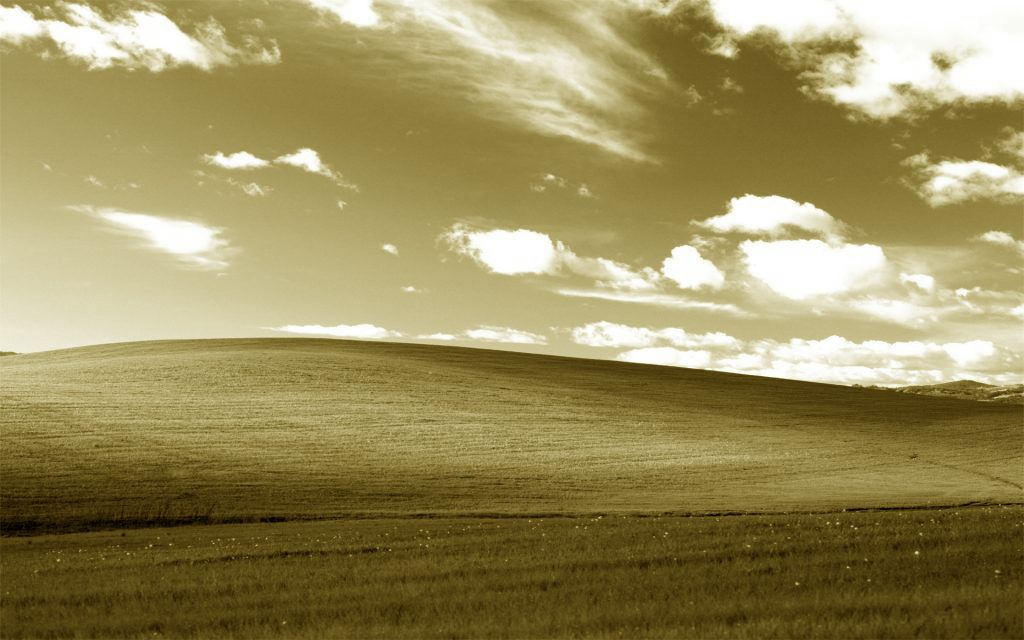
\includegraphics[height=5cm,width=8cm]{D:/Uni/Tex/3.gyakorlat/3.gyakorlat_1feladat/szepia.jpg}
\end{subfigure}
\end{figure}
\hulipsum[1]
\\
\begin{table}[h]
\caption{1}
\centering
\begin{tabular}{|l|c|r|p{30pt}}
\cline{1-3}
rövid szöveg&rövid szöveg&rövid szöveg
\\ \hline
rövid szöveg&&
\\ \hline
rövid szöveg&&
\\ \hline
rövid szöveg&&
\\ \hline
\end{tabular}
\end{table}
\begin{table}[h]
\centering
\caption{2.a}
\begin{tabular}{|c|r|p{30pt}}
\cline{1-2}
\rowcolor{gray}
a&a
\\ \hline
\rowcolor{red}
a&
\\ \hline
\rowcolor{green}
a&
\\ \hline
\rowcolor{blue}
a&
\\ \hline
\end{tabular}
\end{table}
\begin{table}[h]
\centering
\caption{2.b}
\begin{tabular}{|>{\columncolor{gray}}c!{\color{red}\vrule}>{\columncolor{black}}r|p{30pt}}
\cline{1-2}
\cellcolor{red}a&\cellcolor{gray}a
\\ \arrayrulecolor{green}\hline
a&\textcolor{white}{a}
\\ \arrayrulecolor{black}\hline
a&\textcolor{white}{a}
\\ \arrayrulecolor{orange}\hline
a&\textcolor{white}{a}
\\ \arrayrulecolor{pink}\hline
\end{tabular}
\end{table}
\clearpage
\begin{table}[h]
\begin{wrapfigure}[5]{L}[\marginparwidth]{1.5cm}
\caption{3}
\begin{tabular}{|c|r|p{30pt}}
\cline{1-2}
\multicolumn{2}{|c|}{a}
\\ \hline
a&a
\\ \hline
\multirow{2}{1em}{a}&a
\\
&a
\\ \hline
\end{tabular}
\end{wrapfigure}
\hulipsum[1]
\end{table}
\verb|Ez egy sima szöveg \bfseries{ahol ezt a kódot használnám}|
\begin{verbatim}
\begin{enumerate}
        \item Egy
        \item Kettő
        \item Három
\end{enumerate}
\end{verbatim}
\begin{lstlisting}[language=python,tabsize=2,showspaces=false,showtabs=false,numbers=left,stepnumber=4,frame=single,framexleftmargin=20pt]
def binary_search(arr, val, start, end):
	if start == end:
		if arr[start] > val:
			return start
		else:
			return start+1
	elif start > end:
		return start
	else: 
		mid = (start+end)/2
		if arr[mid] < val:
			return binary_search(arr, val, mid+1, end)
		elif arr[mid] > val:
			return binary_search(arr, val, start, mid-1)
		else: # arr[mid] = val
			return mid
			
def insertion_sort(arr):
    for i in xrange(1, len(arr)):
        val = arr[i]
        j = binary_search(arr, val, 0, i-1)
        arr = arr[:j] + [val] + arr[j:i] + arr[i+1:]
    return arr
\end{lstlisting}
\clearpage
\lstset{tabsize=2,showspaces=false,showtabs=false,numbers=left,stepnumber=4,framexleftmargin=20pt}
%\lstinputlisting[language=c,backgroundcolor=\color{gray!20},keywordstyle=\color{red!50!black},identifierstyle=\color{blue!50!black},commentstyle=\color{gray},language=c]{D:/Uni/Tex/3.gyakorlat/3.gyakorlat_1feladat/binsearch.c}%
\begin{lstlisting}[float=hb!,caption={Python},language=python,tabsize=2,showspaces=false,showtabs=false,numbers=left,stepnumber=4,frame=single,framexleftmargin=20pt]
def binary_search(arr, val, start, end):
	if start == end:
		if arr[start] > val:
			return start
		else:
			return start+1
	elif start > end:
		return start
	else: 
		mid = (start+end)/2
		if arr[mid] < val:
			return binary_search(arr, val, mid+1, end)
		elif arr[mid] > val:
			return binary_search(arr, val, start, mid-1)
		else: # arr[mid] = val
			return mid
			
def insertion_sort(arr):
    for i in xrange(1, len(arr)):
        val = arr[i]
        j = binary_search(arr, val, 0, i-1)
        arr = arr[:j] + [val] + arr[j:i] + arr[i+1:]
    return arr
\end{lstlisting}
\begin{lstlisting}[float=hb!,caption={C nyelv},language=c,tabsize=2,showspaces=false,showtabs=false,numbers=left,stepnumber=4,frame=single,framexleftmargin=20pt]
// this is just a code snippet saved from the internet
// for LaTeX code input testing

binarySearch(arr, x, low, high)
	repeat till low = high
		mid = (low + high)/2
			if (x == arr[mid])
				return mid

			else if (x > arr[mid])	// x is on the right side
				low = mid + 1

			else			// x is on the left side
				high = mid - 1

recursiveBinarySearch(arr, x, low, high)
	if low > high
		return False

	else
		mid = (low + high) / 2
		if x == arr[mid]
			return mid

		else if x > arr[mid]	// x is on the right side
			return binarySearch(arr, x, mid + 1, high)

		else			// x is on the left side
			return binarySearch(arr, x, low, mid - 1)

// ok bye
\end{lstlisting}
\end{document}
